

\subsection{Effects / Reverb}
\label{subsec:effects_edit_reverb}

   A Reverberation actually expresses the effect of many echoes being played
   at the same time. This can happen in an enclosed room, where the sound can
   be reflected in different angles. Also, in nature, thunders approximate
   reverbs, because the sound is reflected in many different ways, arriving
   at the listener at different times.

   In music, reverbs are popular in many ways. Reverbs with large room size
   can be used to emulate sounds like in live concerts. This is useful for
   voices, pads, and hand claps. A small room size can simulate the sound
   board of string instruments, like guitars or pianos.

\subsubsection{Effects / Reverb / Circuit}
\label{subsubsec:effects_edit_reverb_circuit}

   As mentioned, a reverb consists of permanent echo. The reverb in
   ZynAddSubFX is more complex than the echo. After the delaying, comb
   filters and then allpass filters are being applied. These make the
   resulting sound more realistic. The parameters for these filters depend on
   the roomsize. For details, consider the information about Freeverb.

\begin{figure}[H]
   \centering 
   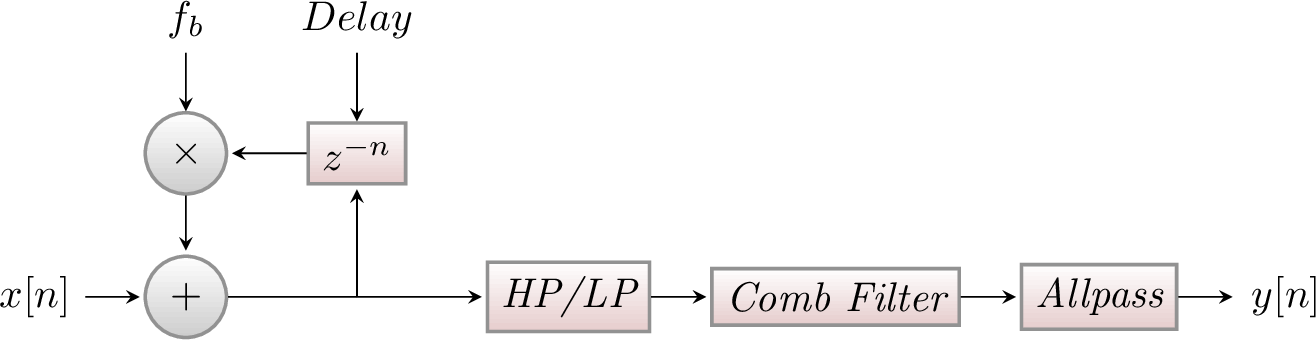
\includegraphics[scale=0.25]{zyn/effects/reverb.png}
   \caption{Reverb Circuit Diagram}
   \label{fig:reverb_circuit_diagram}
\end{figure}

\subsubsection{Effects / Reverb / User Interface}
\label{subsubsec:effects_edit_reverb_ui}

   The user-interface for the Reverb effect depends on whether it is used as a
   System effect or an Insertion effect.
   In \figureref{fig:effects_edit_reverb},
   the Insertion mode is shown.  In the System mode, only the light-blue
   portion of the user-interface appears.

\begin{figure}[H]
   \centering 
   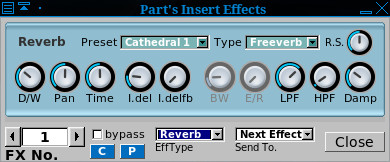
\includegraphics[scale=1.0]{bottom-panel/instrument-edit/Effects/effects-edit-reverb.jpg}
   \caption{Effects Edit, Reverb}
   \label{fig:effects_edit_reverb}
\end{figure}

   \begin{enumber}
      \item \textbf{Preset}
      \item \textbf{Type}
      \item \textbf{R.S.}
      \item \textbf{D/W}
      \item \textbf{Pan}
      \item \textbf{Time}
      \item \textbf{I.del}
      \item \textbf{I.delfb}
      \item \textbf{BW}
      \item \textbf{E/R}
      \item \textbf{LPF}
      \item \textbf{HPF}
      \item \textbf{Damp}
      \item \textbf{FX No.}
      \item \textbf{bypass}
      \item \textbf{EffType}
      \item \textbf{Send To}
      \item \textbf{C}
      \item \textbf{P}
      \item \textbf{Close}
   \end{enumber}

   DID WE CONFUJSE PHASER AND REVEB?

   Note that "FX No.", "bypass", "EffType", "Send To", "C", and "P" are only
   shown if the effect is used as an Insertion effect, not a System Effect.

   \setcounter{ItemCounter}{0}      % Reset the ItemCounter for this list.

   \itempar{Preset}{reverb!preset}
      Reverb Preset.

\begin{figure}[H]
   \centering 
   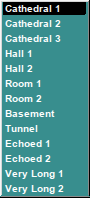
\includegraphics[scale=1.0]{bottom-panel/instrument-edit/Effects/reverb-preset-dropdown.png}
   \caption{Reverb Preset Dropdown}
   \label{fig:reverb_preset_dropdown}
\end{figure}

   Values: \texttt{Cathedral 1, Cathedral 2, Cathedral 3, Half 1, Half 2,

   \itempar{Depth}{reverb!depth}
   Reverb Depth.

   \itempar{Phase}{reverb!phase}
   Reverb Phase.

   \itempar{Stages}{reverb!stagges}
   Reverb Stages.
   How many times the phase is shifted.

   \itempar{Subtract}{reverb!subtract}
   Reverb Subtract.

   \itempar{hyper}{reverb!hyper}
   Reverb Hyper.

   \itempar{Analog}{reverb!analog}
   Reverb Analog.

   \itempar{D/W}{reverb!d/w}
   Reverb Dry/Wet.

   \itempar{Pan}{reverb!pan}
   Reverb Pan.

   \itempar{Freq}{reverb!freq}
   Reverb Freq.

   \itempar{Rnd}{reverb!randomness}
   Reverb Randomness.

   \itempar{St.df}{reverb!st.df}
   The phase difference between LFO for left/right channels.

   \itempar{Fb}{reverb!Fb}
   Reverb Feedback.

   \itempar{L/R}{reverb!L/R}
   Reverb Left/Right.
   Sets how the left/right channels are routed to output:

      \begin{itemize}
         \item Leftmost. Left to left and right to right.
         \item Middle. Left+right to mono.
         \item Rightmost. Left to right, and right to left.
      \begin{itemize}

   \itempar{dist}{reverb!dist}
   Reverb Distortion? TODO

   \itempar{LFO}{reverb!LFO TYpe}
   Reverb LFO Type.
